\begin{figure}[p]
\centering
\renewcommand{\arraystretch}{1.05}
\begin{tabular}{@{}p{\dimexpr(\textwidth-6\tabcolsep)/3\relax}p{\dimexpr(\textwidth-6\tabcolsep)/3\relax}p{\dimexpr(\textwidth-6\tabcolsep)/3\relax}@{}}
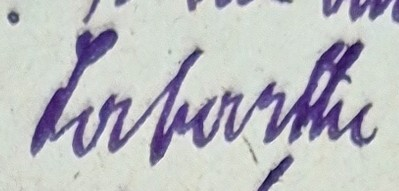
\includegraphics[width=0.96\linewidth,height=12.6mm,keepaspectratio]{illustrations/planche/01_057.jpg} & 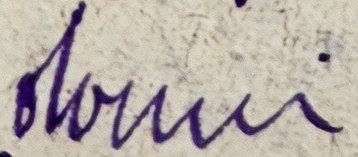
\includegraphics[width=0.96\linewidth,height=12.6mm,keepaspectratio]{illustrations/planche/02_049.jpg} & 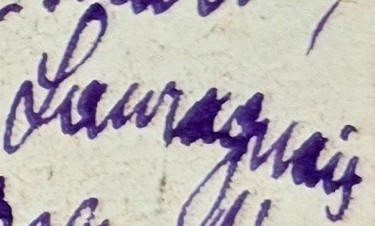
\includegraphics[width=0.96\linewidth,height=12.6mm,keepaspectratio]{illustrations/planche/03_057.jpg} \\
{\scriptsize a fermé, b bouclé — Labarthe \textcolor{LJgris}{(f.~29~r\textsuperscript{o})}} & {\scriptsize d bouclé en arrière — dormi \textcolor{LJgris}{(f.~25~r\textsuperscript{o})}} & {\scriptsize s final plongeant — Lauraguais \textcolor{LJgris}{(f.~29~r\textsuperscript{o})}} \\[1.2mm]
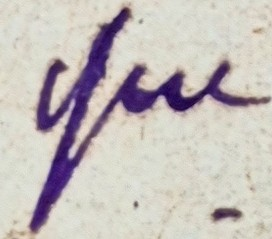
\includegraphics[width=0.96\linewidth,height=12.6mm,keepaspectratio]{illustrations/planche/04_071.jpg} & 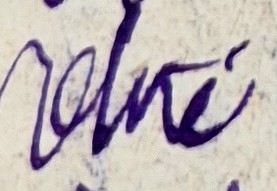
\includegraphics[width=0.96\linewidth,height=12.6mm,keepaspectratio]{illustrations/planche/05_049.jpg} & 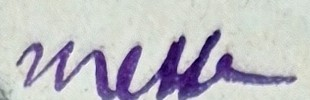
\includegraphics[width=0.96\linewidth,height=12.6mm,keepaspectratio]{illustrations/planche/06_060.jpg} \\
{\scriptsize q à haste droite — que \textcolor{LJgris}{(f.~36~r\textsuperscript{o})}} & {\scriptsize r initial bouclé — retiré \textcolor{LJgris}{(f.~25~r\textsuperscript{o})}} & {\scriptsize ss montants (« ll ») — messe \textcolor{LJgris}{(f.~30~v\textsuperscript{o})}} \\[1.2mm]
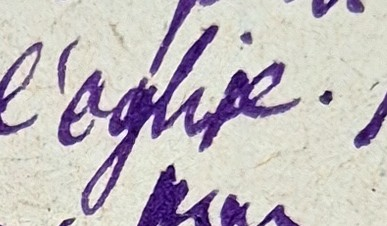
\includegraphics[width=0.96\linewidth,height=12.6mm,keepaspectratio]{illustrations/planche/07_057.jpg} & 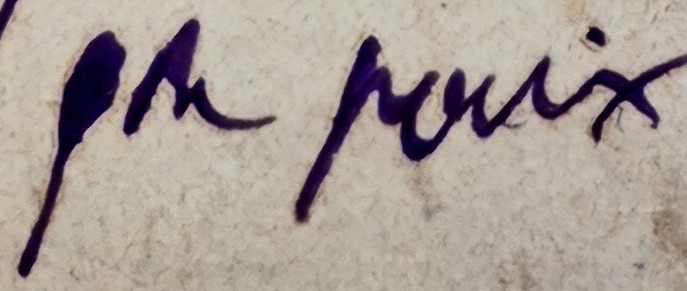
\includegraphics[width=0.96\linewidth,height=12.6mm,keepaspectratio]{illustrations/planche/08_071.jpg} & 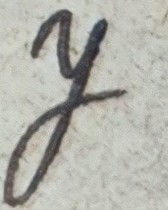
\includegraphics[width=0.96\linewidth,height=12.6mm,keepaspectratio]{illustrations/planche/09_041.jpg} \\
{\scriptsize g et s long descendants — l'église \textcolor{LJgris}{(f.~29~r\textsuperscript{o})}} & {\scriptsize g\textsuperscript{de}, x en croix — gde paix \textcolor{LJgris}{(f.~36~r\textsuperscript{o})}} & {\scriptsize y à tête en V — y \textcolor{LJgris}{(f.~21~r\textsuperscript{o})}} \\[1.2mm]
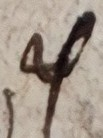
\includegraphics[width=0.96\linewidth,height=12.6mm,keepaspectratio]{illustrations/planche/10_014.jpg} & 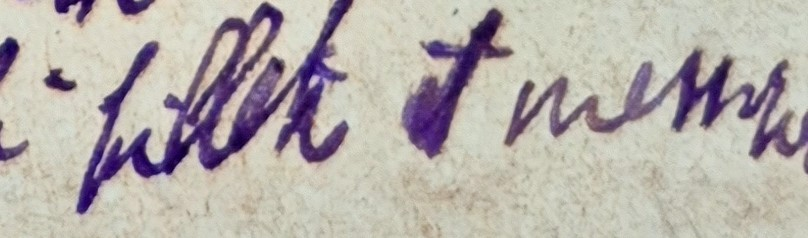
\includegraphics[width=0.96\linewidth,height=12.6mm,keepaspectratio]{illustrations/planche/11_090.jpg} & 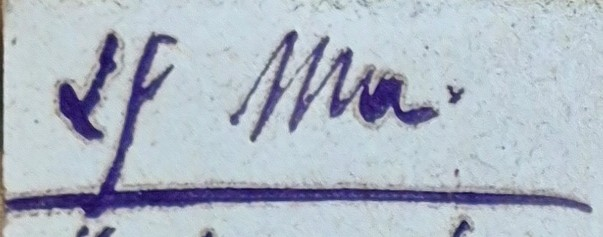
\includegraphics[width=0.96\linewidth,height=12.6mm,keepaspectratio]{illustrations/planche/12_002.jpg} \\
{\scriptsize esperluette « en 4 » — \& \textcolor{LJgris}{(f.~7~v\textsuperscript{o})}} & {\scriptsize \& en « t bouclé » — billets \& mess \textcolor{LJgris}{(f.~45~v\textsuperscript{o})}} & {\scriptsize date soulignée, 5 à drapeau — 25 Ma. \textcolor{LJgris}{(f.~1~r\textsuperscript{o})}} \\[1.2mm]
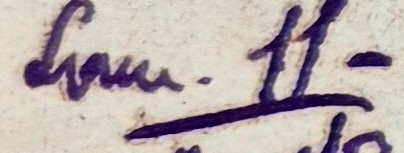
\includegraphics[width=0.96\linewidth,height=12.6mm,keepaspectratio]{illustrations/planche/13_097.jpg} & 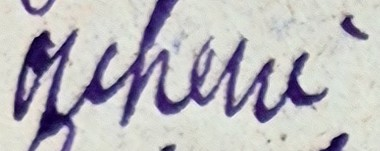
\includegraphics[width=0.96\linewidth,height=12.6mm,keepaspectratio]{illustrations/planche/14_049.jpg} & 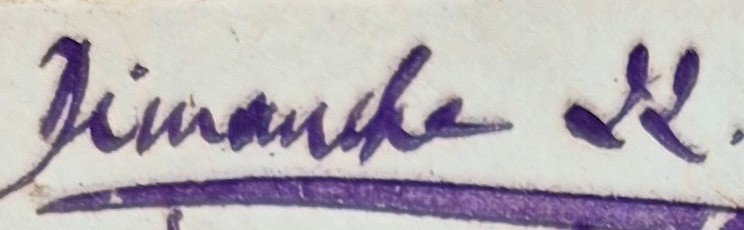
\includegraphics[width=0.96\linewidth,height=12.6mm,keepaspectratio]{illustrations/planche/15_083.jpg} \\
{\scriptsize S en L bouclé, tiret — Sam. 11 — \textcolor{LJgris}{(f.~48~v\textsuperscript{o})}} & {\scriptsize A cursif (a agrandi) — Achevé \textcolor{LJgris}{(f.~25~r\textsuperscript{o})}} & {\scriptsize D en J, 2 bouclé — Dimanche 22. \textcolor{LJgris}{(f.~42~r\textsuperscript{o})}} \\[1.2mm]
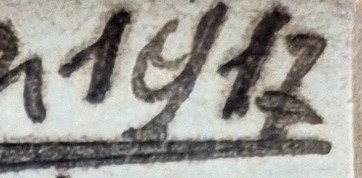
\includegraphics[width=0.96\linewidth,height=12.6mm,keepaspectratio]{illustrations/planche/16_124.jpg} & 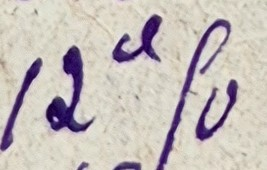
\includegraphics[width=0.96\linewidth,height=12.6mm,keepaspectratio]{illustrations/planche/17_053.jpg} & 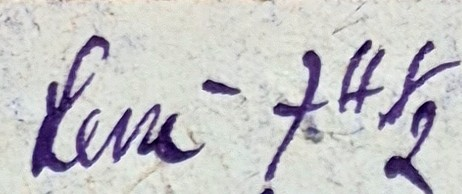
\includegraphics[width=0.96\linewidth,height=12.6mm,keepaspectratio]{illustrations/planche/18_049.jpg} \\
{\scriptsize 7 barré — 1917 \textcolor{LJgris}{(f.~62~r\textsuperscript{o})}} & {\scriptsize f suscrit, 5 bouclé — 12\textsuperscript{f} 50 \textcolor{LJgris}{(f.~27~r\textsuperscript{o})}} & {\scriptsize H suscrit, demi — Levé – 7\textsuperscript{H}\LJfrac{1}{2} \textcolor{LJgris}{(f.~25~r\textsuperscript{o})}} \\[1.2mm]
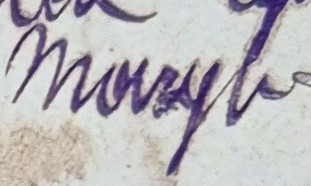
\includegraphics[width=0.96\linewidth,height=12.6mm,keepaspectratio]{illustrations/planche/19_002.jpg} & 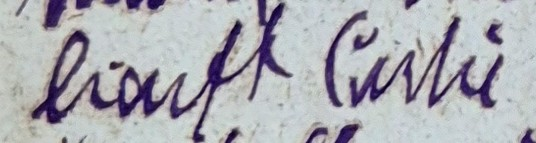
\includegraphics[width=0.96\linewidth,height=12.6mm,keepaspectratio]{illustrations/planche/20_002.jpg} & 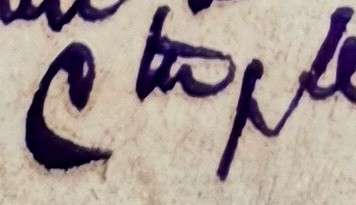
\includegraphics[width=0.96\linewidth,height=12.6mm,keepaspectratio]{illustrations/planche/21_097.jpg} \\
{\scriptsize Marg\textsuperscript{te} (Marguerite) \textcolor{LJgris}{(f.~1~r\textsuperscript{o})}} & {\scriptsize lieut\textsuperscript{t} Curtis \textcolor{LJgris}{(f.~1~r\textsuperscript{o})}} & {\scriptsize C\textsuperscript{tes} p\textsuperscript{les} (cartes postales) \textcolor{LJgris}{(f.~48~v\textsuperscript{o})}} \\[1.2mm]
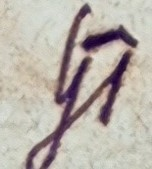
\includegraphics[width=0.96\linewidth,height=12.6mm,keepaspectratio]{illustrations/planche/22_076.jpg} & 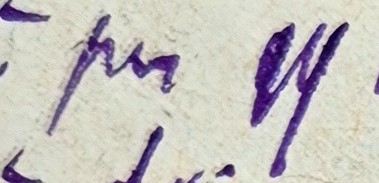
\includegraphics[width=0.96\linewidth,height=12.6mm,keepaspectratio]{illustrations/planche/23_060.jpg} & 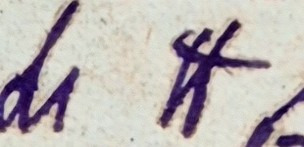
\includegraphics[width=0.96\linewidth,height=12.6mm,keepaspectratio]{illustrations/planche/24_076.jpg} \\
{\scriptsize tjs (toujours) \textcolor{LJgris}{(f.~38~v\textsuperscript{o})}} & {\scriptsize pr (pour) ; qq (quelques) \textcolor{LJgris}{(f.~30~v\textsuperscript{o})}} & {\scriptsize ds (dans) ; tt (tout) \textcolor{LJgris}{(f.~38~v\textsuperscript{o})}} \\[1.2mm]
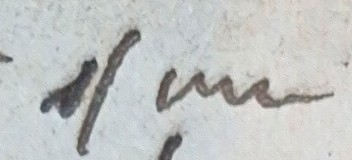
\includegraphics[width=0.96\linewidth,height=12.6mm,keepaspectratio]{illustrations/planche/25_007.jpg} & 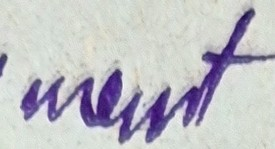
\includegraphics[width=0.96\linewidth,height=12.6mm,keepaspectratio]{illustrations/planche/26_060.jpg} & 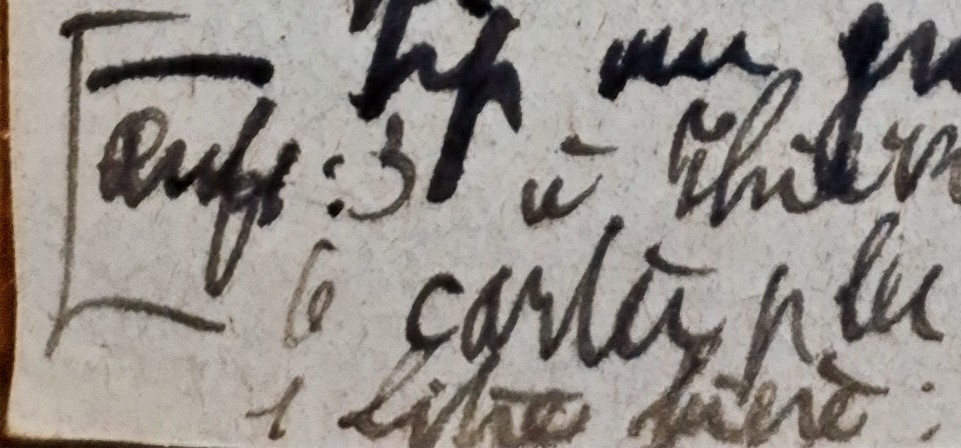
\includegraphics[width=0.96\linewidth,height=12.6mm,keepaspectratio]{illustrations/planche/27_041.jpg} \\
{\scriptsize s/ (sur) — s/ une \textcolor{LJgris}{(f.~3~v\textsuperscript{o})}} & {\scriptsize merv\textsuperscript{t} (merveilleusement) \textcolor{LJgris}{(f.~30~v\textsuperscript{o})}} & {\scriptsize crochet de comptes (3 lignes) \textcolor{LJgris}{(f.~21~r\textsuperscript{o})}} \\[1.2mm]
\end{tabular}
\caption{Planche paléographique : formes caractéristiques de l'écriture d'Hippolyte Combes (1916–1917)}
\label{planche}
\end{figure}